% V3: control policy refiner with the solver as decoder (cost weights -> Riccati gains), up to 6 pages.
% Based on the IEEE conference template (IEEEtran, conference mode), with small deviations
% (author block with advisors, tighter floats).
\documentclass[conference]{IEEEtran}
\IEEEoverridecommandlockouts
\usepackage{cite}
\usepackage{amsmath,amssymb,amsfonts}
\usepackage{graphicx}
\usepackage{textcomp}
\usepackage{xcolor}
\usepackage{booktabs}
\usepackage{url}
\usepackage{tikz}
\usetikzlibrary{arrows.meta,positioning,calc,fit}

\newcommand{\R}{\mathbb{R}}
\newcommand{\T}{^{\top}}
\newcommand{\mpc}{\mathrm{MPC}}
\newcommand{\xb}{\bar{x}}
\newcommand{\ub}{\bar{u}}
\setlength{\textfloatsep}{9pt plus 2pt minus 2pt}
\setlength{\dbltextfloatsep}{9pt plus 2pt minus 2pt}
\setlength{\abovecaptionskip}{3pt}

\begin{document}

\title{Control Policy Refiner in Legged Robotics:\\ Preliminary Results}

\author{\IEEEauthorblockN{Norawit Nangsue\textsuperscript{1,2}}
\IEEEauthorblockA{Advisors: Fumio Kanehiro\textsuperscript{1,2} and Mehdi Benallegue\textsuperscript{2}}
\IEEEauthorblockA{\textsuperscript{1}University of Tsukuba, Ibaraki, Japan\\
\textsuperscript{2}CNRS-AIST JRL (Joint Robotics Laboratory), IRL,\\
National Institute of Advanced Industrial Science and Technology (AIST), Japan}}

\maketitle

\begin{abstract}
A model predictive controller (MPC) based on differential dynamic programming provides a feedback policy, made of a state set-point and a gain matrix, that drives a humanoid robot between two solves.
This controller is optimal for under model assumption, not the real-world robot.
We propose a \emph{control policy refiner} that makes the robot more robust to uncertainty by outputting differential to gain and set-point to improve the overall performance.
Modifying gain space directly directly leads to dimensionality problem. Therefore, we decided to devise a network that output the latent representation and feed to the solver, which effectively become a decoder. One Riccati backward pass along the current trajectory turns the modified weights into a full gain matrix.
Every gain and setpoint deviation from the refiner is therefore the optimal feedback of a local problem, which keeps exploration safe and small.
For the base controller, we implemented an IS-MPC gait generator with a reformulated footstep timing and position pre-optimization and a whole-body MPC of HRP-5P legs.
In MuJoCo it walks at up to 0.3\,m/s with a mean whole-body solve time of 6.7\,ms and recovers from 26 of 36 pushes.
The refiner itself has not been trained yet.
\end{abstract}

\begin{IEEEkeywords}
humanoid robots, model predictive control, residual reinforcement learning, feedback gain modification, set-point modification
\end{IEEEkeywords}

\section{Introduction}

Model-based walking controllers for humanoid robots are commonly built in two layers.
The upper layer plans with a reduced model, such as the linear inverted pendulum (LIPM) \cite{kajita2001lipm,kajita2003preview}, and the lower layer can either be a whole-body controller which computes each joint torque at each moment and may be implemented as whole-body MPC \cite{mastalli2020crocoddyl,dantec2022wbmpc}.

This division makes model-based walking fast enough to be used in practice and the reduced model can be analyzed thoroughly.

A control law that prevents from falling, by adjusting the zero-moment point (ZMP) and footsteps so that the unstable part of the LIPM dynamics known as Divergent component of motion (DCM) \cite{takenaka2009dcm,englsberger2011capture} can be derived from the model and evaluated.
This concept is formulated in a closed form knownas the boundedness condition \cite{lanari2014boundedness} and a family of algorithm that apply this concept called IS-MPC\cite{scianca2020ismpc,dallard2025adios} utilize this equation as constraint such that the robot can properly balance forever.

Once the balance is handled by the of the reduced model, the whole-body controller has a guide on how to walk properly given, the center of mass (CoM), foot and contact references.

However, this approach is best under the model assumption; it does not take model mismatching and uncertainties into consideration.
On the otherhands, learning-based controllers, which train a neural network policy in simulation with reinforcement learning (RL) \cite{hwangbo2019learning,radosavovic2024humanoid}, can adapt to such effects from experience, but they are black boxes which may be subject to safety concern and explanability.

The idea of combining the both approaches is called Residual RL \cite{silver2018residual,johannink2019residual}. The model-based controller is kept and a learned correction is added to its output, as a joint torque or a position target \cite{jenelten2024dtc,jeon2025residualmpc}.

Nevertheless, residual reinforcement learning is not meant to always provide the signal at the output only; solving MPC problem with differential dynamic programming (DDP) \cite{mayne1966ddp} may allow us to modify even the tracking controller.
The DDP solver returns Riccati gains, set-point and the torque trajectory that drives the robot between two solves.
In existing work these gains are applied as computed.
Our goal is to make this feedback policy robust to uncertainty by letting a learned policy, the \emph{refiner}, adjust it online.
It turns out learning the gains directly may not be practical: for the leg model they have 432 entries per node, and an arbitrary change can destabilize the robot.
We instead let the refiner act on the \emph{cost} from which the gains are computed, and we use the solver as a decoder, effectively reduce the learning variable to X

This paper presents (i) the base controller (Section~\ref{sec:base}), (ii) the refiner and its decoder (Section~\ref{sec:method}), (iii) simulation results of the base controller that show what has to be corrected (Section~\ref{sec:results}), and (iv) the plan (Section~\ref{sec:plan}).

\section{Related Work}

\emph{Gait generation with reduced models.}
The LIPM underlies preview control \cite{kajita2003preview} and the linear MPC gait generators that also choose the footsteps \cite{wieber2006mpc,herdt2010online}.
IS-MPC \cite{scianca2020ismpc} enforces the boundedness condition of \cite{lanari2014boundedness} as a constraint, and Dallard \emph{et al.} \cite{dallard2025adios} closed the loop on the measured state and added a pre-optimization of the footstep timing, which is essential for push recovery \cite{khadiv2020timing}.

\emph{Whole-body MPC and Riccati feedback.}
DDP \cite{mayne1966ddp,tassa2012synthesis} solves the whole-body problem fast enough for MPC and has been demonstrated on a torque-controlled humanoid \cite{dantec2022wbmpc}.
Its Riccati gains are a first-order approximation of how the MPC solution changes with the state \cite{dantec2022firstorder}, and they are used to run the feedback at a higher rate than the solver; they must be consistent with the contact constraints to be usable on hardware \cite{grandia2019feedback}.

\emph{RL combined with model-based control.}
A policy can track a model-based plan \cite{jenelten2024dtc,kang2023rlmodel} or correct a model-based controller \cite{cheng2025rambo,jeon2025residualmpc}.
Closer to our approach, a policy can set the parameters of an MPC: the decision variables of a quadrotor MPC \cite{song2022policysearch}, a learned cost in a differentiable MPC \cite{amos2018diffmpc,romero2024acmpc}, or, in theory, any parameter of an MPC used as a policy \cite{gros2020nmpcrl}.
These methods solve the MPC again with the new parameters, which changes the planned motion.
Our refiner keeps the plan and changes only the reaction: the weights are decoded into new gains by one backward pass, between two solves.
This is in the spirit of variable impedance learning \cite{buchli2011variable} and of LQR weight tuning \cite{marco2016lqr}, applied online to the time-varying gains of a whole-body MPC.

\section{Base Controller}
\label{sec:base}

\begin{figure*}[t]
\centering
\resizebox{0.96\textwidth}{!}{%
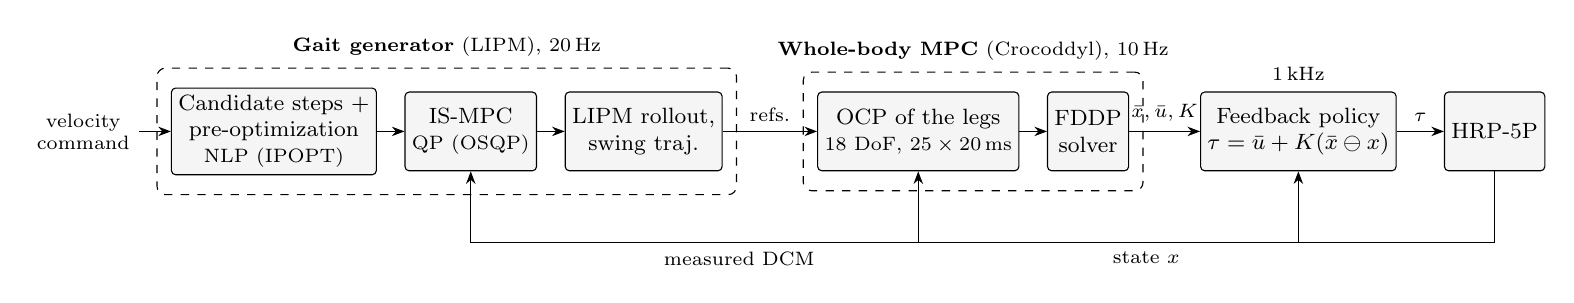
\begin{tikzpicture}[font=\footnotesize, >={Stealth[length=1.6mm]},
  blk/.style={draw, rounded corners=1.5pt, minimum height=10mm, align=center, inner sep=2.5pt, fill=black!4},
  grp/.style={draw, dashed, rounded corners=3pt, inner sep=5pt, inner ysep=7pt},
  lab/.style={font=\scriptsize, align=center}]
\node[lab] (cmd) {velocity\\command};
\node[blk, right=4mm of cmd] (ftpp) {Candidate steps +\\pre-optimization\\{\scriptsize NLP (IPOPT)}};
\node[blk, right=3.5mm of ftpp] (ismpc) {IS-MPC\\{\scriptsize QP (OSQP)}};
\node[blk, right=3.5mm of ismpc] (roll) {LIPM rollout,\\swing traj.};
\node[blk, right=12mm of roll] (ocp) {OCP of the legs\\{\scriptsize 18 DoF, $25\times20$\,ms}};
\node[blk, right=3.5mm of ocp] (ddp) {FDDP\\solver};
\node[blk, right=9mm of ddp] (ric) {Feedback policy\\$\tau=\ub+K(\xb\ominus x)$};
\node[blk, right=6mm of ric] (rob) {HRP-5P};
\node[grp, fit=(ftpp)(ismpc)(roll)] (gg) {};
\node[grp, fit=(ocp)(ddp)] (wb) {};
\node[lab, above=0.2mm of gg.north] {\textbf{Gait generator} (LIPM), 20\,Hz};
\node[lab, above=0.2mm of wb.north] {\textbf{Whole-body MPC} (Crocoddyl), 10\,Hz};
\node[lab, above=0.2mm of ric.north] {1\,kHz};
\draw[->] (cmd) -- (ftpp);
\draw[->] (ftpp) -- (ismpc);
\draw[->] (ismpc) -- (roll);
\draw[->] (roll) -- node[lab, above] {refs.} (ocp);
\draw[->] (ocp) -- (ddp);
\draw[->] (ddp) -- node[lab, above] {$\xb,\ub,K$} (ric);
\draw[->] (ric) -- node[lab, above] {$\tau$} (rob);
\coordinate (fb) at ($(ric.south)+(0,-9mm)$);
\draw[->] (rob.south) |- (fb) -- (ric.south);
\draw[->] (fb) -| node[lab, pos=0.2, below] {state $x$} (ocp.south);
\draw[->] (fb -| ocp.south) -| node[lab, pos=0.2, below] {measured DCM} (ismpc.south);
\end{tikzpicture}}
\caption{Base controller: an IS-MPC gait generator sends CoM, foot and contact references to a whole-body MPC built on Crocoddyl, whose feedback policy is evaluated at 1\,kHz on HRP-5P model in MuJoCo.}
\label{fig:base}
\end{figure*}

\begin{figure}[t]
\centering
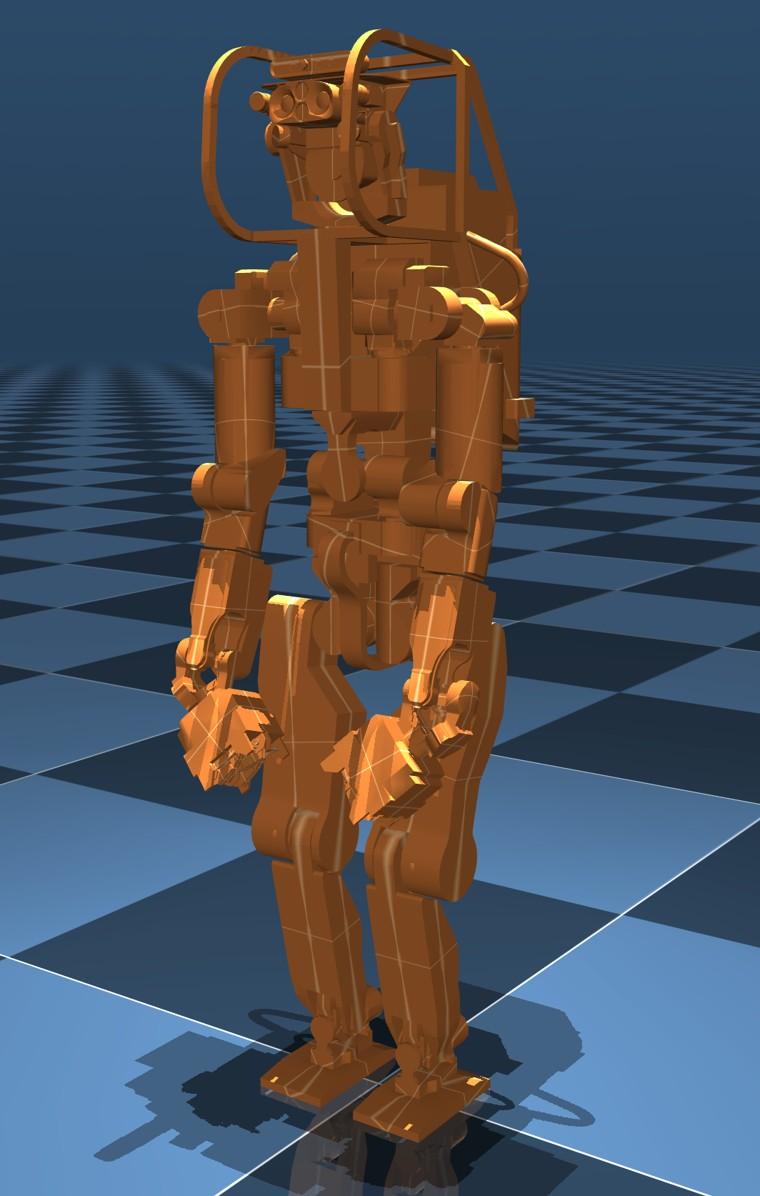
\includegraphics[width=0.42\columnwidth]{figures/hrp5p.jpg}
\caption{HRP-5P model in MuJoCo, in the standing posture from which all runs start.}
\label{fig:robot}
\end{figure}

\subsection{Gait generator}
With CoM $c$, ZMP $p$ and $\eta=\sqrt{g/z_c}$ for a constant CoM height $z_c$, the LIPM is $\ddot c=\eta^2(c-p)$.
The DCM $\xi=c+\dot c/\eta$ splits it into a stable and an unstable first-order system,
\begin{equation}
\dot c=\eta(\xi-c),\qquad \dot\xi=\eta(\xi-p).
\label{eq:dcm}
\end{equation}
The CoM follows the DCM, and the DCM diverges from the ZMP.
It stays bounded if and only if \cite{lanari2014boundedness}
\begin{equation}
\xi(t_0)=\eta\int_{0}^{\infty}e^{-\eta\tau}\,p(t_0+\tau)\,d\tau .
\label{eq:stab}
\end{equation}
The initial DCM cannot be chosen, so \eqref{eq:stab} is a constraint on the future ZMP.
IS-MPC \cite{scianca2020ismpc} enforces it in a QP on the ZMP velocity and the footsteps, with the ZMP kept inside the support region.

After a push, \eqref{eq:stab} may be infeasible with the nominal step times, so the footstep positions $p_f^k$ and times $t_k$ are first adjusted by a pre-optimization \cite{dallard2025adios}.
Integrating \eqref{eq:stab} piecewise over the steps shows that the DCM must lie in a sum of the support regions weighted by $\mu_k-\mu_{k+1}$, with $\mu_k=e^{-\eta t_k}$; a slack $s$ measures by how much this condition is violated.
This problem is badly scaled, since $\mu_k$ reaches $10^{-7}$ at the end of the preview, and the reference implementation \cite{ismpcwalking} solves it by block coordinate descent between positions and times, dropping the divisor of the displacement term.
We replace $\mu_k$ by the ratio $\nu_k=\mu_k/\hat\mu_k$ to its nominal value, which makes all variables of order one, keep the original cost
\begin{multline}
J=\sum_k(\nu_k-1)^2+w_s\|s\|^2\\
+K_s\sum_{i\ge1}\big\|p_f^i-\hat p_f^i\big\|^2\,
\frac{(\nu_i\hat\mu_i-\nu_{i-1}\hat\mu_{i-1})^2}{(\hat\mu_i-\hat\mu_{i-1})^2},
\label{eq:cost}
\end{multline}
and solve positions and times jointly as one nonlinear program with CasADi \cite{andersson2019casadi} and IPOPT \cite{wachter2006ipopt}.
The program is built once per number of steps and cached, so a replan only runs the solver.

The IS-MPC QP then uses the result as candidates, with a 2.5\,s control horizon, an anticipative tail up to 6\,s and a term that centers the ZMP in the sole, and is solved with OSQP \cite{stellato2020osqp}.
The generator replans at every touchdown and solves the QP again every 50\,ms.
It includes capture steps and a DCM feedback law for standing, and it detects a push and react when the measured DCM jumps by more than 4\,cm from the planned one within one tick.

\subsection{Whole-body MPC and its feedback policy}
The optimal control problem (OCP) uses the floating base and the twelve leg joints of HRP-5P \cite{kaneko2019hrp5p} ($n_v=18$); the upper body is held by a separate joint-space controller.
Contacts are rigid 6D constraints that follow the schedule of the gait generator.
The running cost is a weighted sum of residuals,
\begin{equation}
\ell(x,u)=\tfrac12\sum_{c}w_c\,\|r_c(x,u)\|^2_{W_c},
\label{eq:costwb}
\end{equation}
with terms for the CoM, the feet, the posture (base orientation, joint positions, velocities) and the torques.
The OCP has 25 nodes of 20\,ms and is solved with the FDDP solver of Crocoddyl \cite{mastalli2020crocoddyl} every 100\,ms, with at most ten warm-started iterations.
Each solve returns the trajectories $\xb_i,\ub_i$ and the Riccati gains $K_i$.
Between solves, the torque is
\begin{equation}
\tau^{\mpc}=\ub_i+K_i\,(\xb_i\ominus x),\qquad K_i\in\R^{12\times36},
\label{eq:riccati}
\end{equation}
evaluated at 1\,kHz with the measured state $x$; $\ominus$ is the difference on the state manifold.
The 36 columns of $K_i$ multiply the errors of the base pose (6), the joint positions (12), the base velocity (6) and the joint velocities (12).

\section{Control Policy Refiner}
\label{sec:method}

\begin{figure}[t]
\centering
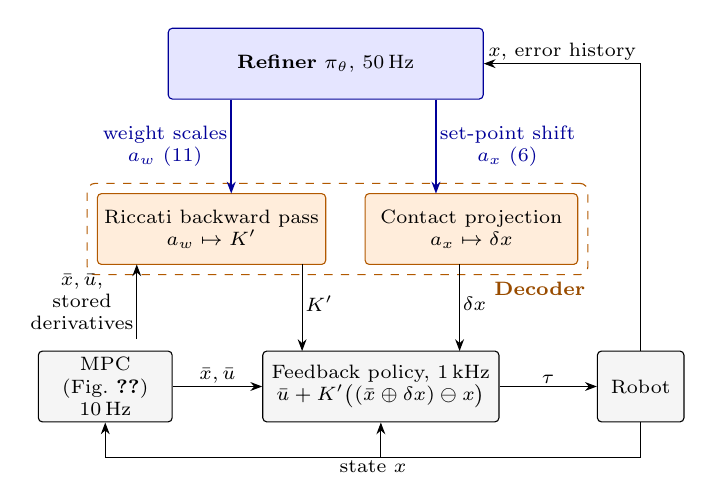
\begin{tikzpicture}[x=1mm, y=1mm, font=\scriptsize, >={Stealth[length=1.5mm]},
  blk/.style={draw, rounded corners=1.5pt, minimum height=9mm, align=center, inner sep=2pt, fill=black!4},
  res/.style={draw, rounded corners=1.5pt, minimum height=9mm, align=center, inner sep=2pt, fill=blue!10, draw=blue!60!black},
  dec/.style={draw, rounded corners=1.5pt, minimum height=9mm, align=center, inner sep=2pt, fill=orange!14, draw=orange!70!black},
  lab/.style={font=\scriptsize, align=center, inner sep=1pt}]
\node[blk, minimum width=17mm] (mpc) at (0,0) {MPC\\(Fig.~\ref{fig:base})\\10\,Hz};
\node[blk, minimum width=30mm] (fb) at (35,0) {Feedback policy, 1\,kHz\\$\ub+K'\big((\xb\oplus\delta x)\ominus x\big)$};
\node[blk, minimum width=11mm] (rob) at (68,0) {Robot};
\node[dec, minimum width=29mm] (bp) at (13.5,20) {Riccati backward pass\\$a_w\mapsto K'$};
\node[dec, minimum width=27mm] (pr) at (46.5,20) {Contact projection\\$a_x\mapsto\delta x$};
\node[draw=orange!70!black, dashed, rounded corners=3pt, inner sep=3.5pt, fit=(bp)(pr)] (decgrp) {};
\node[lab, text=orange!60!black, anchor=north east] at ($(decgrp.south east)+(0,-0.5)$) {\textbf{Decoder}};
\node[res, minimum width=40mm] (pol) at (28,41) {\textbf{Refiner} $\pi_\theta$, 50\,Hz};
\draw[->, blue!60!black, thick] (pol.south -| 16,0) -- node[lab, left, text=blue!60!black] {weight scales\\$a_w$ (11)} (16,24.5);
\draw[->, blue!60!black, thick] (pol.south -| 42,0) -- node[lab, right, text=blue!60!black] {set-point shift\\$a_x$ (6)} (42,24.5);
\draw[->] (4,6) -- node[lab, left] {$\xb,\ub$,\\stored\\derivatives} (4,15.5);
\draw[->] (25,15.5) -- node[lab, right, pos=0.45] {$K'$} (25,4.5);
\draw[->] (45,15.5) -- node[lab, right, pos=0.45] {$\delta x$} (45,4.5);
\draw[->] (mpc) -- node[lab, above] {$\xb,\ub$} (fb);
\draw[->] (fb) -- node[lab, above] {$\tau$} (rob);
\draw[->] (rob.south) -- (68,-9) -| node[lab, pos=0.25, below] {state $x$} (mpc.south);
\draw[->] (68,-9) -| (fb.south);
\draw[->] (rob.north) -- (68,41) -- node[lab, above] {$x$, error history} (pol.east);
\end{tikzpicture}
\caption{The refiner stack. The MPC of Fig.~\ref{fig:base} is treated as one block. The refiner outputs 17 numbers; the decoder turns them into a full gain matrix $K'$, by one backward pass of the solver, and into a contact-consistent set-point shift $\delta x$.}
\label{fig:stack}
\end{figure}

\subsection{Overview}
In \eqref{eq:riccati}, the set-point $\xb$ suggests what state state it should be, and the gain $K$ describes its reactiveness of error through joint torque.
Each MPC solution is executed for 100 control steps, so this law alone determines the behavior in that interval, and it is the law that meets the uncertainty: a push, a wrong mass, a softer floor.
The refiner (Fig.~\ref{fig:stack}) adjusts both parts,
\begin{equation}
\tau=\ub+K'\,\big((\xb\oplus\delta x)\ominus x\big),
\label{eq:refined}
\end{equation}
at the node rate of 50\,Hz.
It outputs a latent $a=(a_w,a_x)$, and a fixed decoder maps $a_w$ to the gain $K'$ and $a_x$ to the shift $\delta x$.
The decoder is not learned: RL explores in the latent, and $a=0$ gives exactly the base controller.
The network is initialized to output zero, so training starts from the behavior of Section~\ref{sec:results}.

\subsection{Solver as decoder for the gains}
The Riccati gains are a function of the cost \eqref{eq:costwb}.
The refiner scales its weights,
\begin{equation}
w_c\leftarrow w_c\,e^{a_{w,c}},
\label{eq:scale}
\end{equation}
and the decoder runs the backward pass of the solver once more along the current trajectory.
With the Gauss--Newton approximation used by the solver, the cost Hessian is linear in the weights, $\ell_{xx}=\sum_c w_c\,J_c\T W_cJ_c$ (and similarly for $\ell_{ux},\ell_{uu}$), so it is a weighted sum of blocks already computed by the last solve.
The dynamics Jacobians $f_x,f_u$ are also stored.
The recursion, from the last node to the first, is
\begin{align}
Q_{uu}&=\ell_{uu}+f_u\T V'_{xx}f_u, &Q_{ux}&=\ell_{ux}+f_u\T V'_{xx}f_x,\nonumber\\
Q_{xx}&=\ell_{xx}+f_x\T V'_{xx}f_x, &K'&=Q_{uu}^{-1}Q_{ux},\nonumber\\
V_{xx}&=Q_{xx}-Q_{ux}\T K', &&
\label{eq:backward}
\end{align}
where $V'_{xx}$ is the value Hessian of the next node.

One pass is enough, and it is not an approximation of a converged solve.
DDP iterates in order to move the trajectory; the gains around a given trajectory are obtained exactly by one backward sweep.
The robot is tracking the trajectory of the last solve, so this is the trajectory around which the gains must be computed.
Only the gains are used: the feedforward torque and the set-point of the last solve are kept, so the decoded gains change the reaction and not the planned motion.

The weight scales are of two kinds (Table~\ref{tab:latent}).
\emph{Tracking weights} set what the feedback protects: the CoM, the base orientation, the joint posture, the velocities (damping) and the feet.
\emph{Torque weights}, one per joint group, set how much each joint is trusted to react: raising the torque weight of the stance ankle softens it, and the rest of the gain adapts so that the hip and the knee take over.
Raising all torque weights lowers the bandwidth of the feedback, which is the classical remedy against unmodeled dynamics.

\begin{table}[t]
\caption{Latent of the refiner}
\label{tab:latent}
\centering
\setlength{\tabcolsep}{3pt}
\resizebox{\columnwidth}{!}{%
\begin{tabular}{@{}llc@{}}
\toprule
Part & Content & Size\\
\midrule
$a_w$, tracking & CoM, base orientation, posture, velocities, feet & 5\\
$a_w$, torque & hip, knee, ankle of the stance and the swing leg & 6\\
$a_x$ & base pose shift; leg joints by contact projection & 6\\
\midrule
\multicolumn{2}{@{}l}{Decoded: $K'\in\R^{12\times36}$ per node, and $\delta x\in\R^{36}$} & 17\\
\bottomrule
\end{tabular}}
\end{table}

\subsection{Set-point shift}
The shift is output directly, restricted to configurations that keep the stance feet in place:
\begin{equation}
\delta x=\begin{bmatrix}P_c\,S\,a_x\\ 0\end{bmatrix},\qquad P_c=I-J_c^{+}J_c ,
\label{eq:setpoint}
\end{equation}
where $S$ selects the base pose and $J_c$ is the Jacobian of the feet in contact, so the refiner outputs a change of the base pose and the projection completes the leg joints.
A shift that moved a stance foot would only create internal forces.
The resulting torque $K'\delta x$ lies in the range of the gain.
Since the Riccati policy is the first-order expansion of the MPC solution with respect to the state \cite{dantec2022firstorder}, it is the torque the MPC itself would command if the robot were displaced by $-\delta x$: the refiner acts as a learned bias on the state seen by the controller.
The shift also enters a loop that is already closed.
With $\zeta_i=x_i\ominus\xb_i$ and $A_i,B_i$ the dynamics Jacobians,
\begin{equation}
\zeta_{i+1}=(A_i-B_iK'_i)\,\zeta_i+B_iK'_i\,\delta x_i ,
\label{eq:cl}
\end{equation}
so a bounded shift gives a bounded deviation as long as the gains stabilize the local model.
The shift handles what a gain cannot, namely steady errors such as a CoM offset.

\subsection{Properties and limits}
\emph{Safe by construction.} With positive weights, $Q_{uu}$ is positive definite and $K'$ is the optimal feedback of a valid local linear-quadratic problem.
The refiner can choose a poor cost, but it cannot produce a gain with flipped signs or with a broken coupling between joints.
$K'$ is also consistent with the contacts, because it is computed through the same contact-constrained dynamics, which is a condition for using such gains on hardware \cite{grandia2019feedback}.

\emph{Small and meaningful.} The latent has 17 numbers, each with a physical meaning that can be bounded and inspected, and the decoded gain depends smoothly on it.

\emph{Cheap.} The decoder is a weighted sum and one recursion over 25 nodes, without new derivatives; a complete solver iteration takes about 0.8\,ms in our implementation, which bounds its cost.

\emph{Limits.} The decoder only reaches gains that are optimal for some cost on the model's dynamics.
If the dynamics themselves are wrong, the best gain may lie outside this family, and the refiner can then only detune.
The gains do not respond evenly to the weights, so the bound of each scale must be calibrated, and the scales are rate-limited, because a fast-varying gain can destabilize a loop even when every frozen value is stabilizing.
The refiner cannot change the footsteps or the contact schedule: disturbances that need a different step remain the task of the gait generator.

\subsection{Learning for robustness}
The refiner observes the state, a short history of tracking errors and torques, the contact flags and the step phase, the velocity command and its previous output.
The history lets it recognize the situation, for example a heavier robot or a softer floor, and choose the weights accordingly, instead of learning one compromise setting.
It is trained with PPO \cite{schulman2017ppo} in simulation under the uncertainties it should withstand: pushes, mass and CoM offsets, friction, contact stiffness and actuation delay.
The reward combines velocity tracking and staying upright with penalties on the size and the rate of the latent, on joint torques, on a center of pressure (CoP) near the sole edge and on a tilted stance foot.
The MPC and the decoder are part of the environment, so no derivative of the solver is needed.

\section{Preliminary Results: Base Controller}
\label{sec:results}

The refiner has not been trained; this section reports the base controller alone, to establish the baseline and to identify what has to be corrected.

\subsection{Setup}
HRP-5P model (104\,kg) is simulated in MuJoCo \cite{todorov2012mujoco} with a 1\,ms step and torque control.
The LIPM height is the measured CoM height when the MPC starts ($z_c=1.014$\,m, $\eta=3.11$\,s$^{-1}$), steps last at most 0.8\,s, and the commands are limited to 0.3\,m/s and 0.3\,rad/s.
Runs are headless on one thread of a laptop (Apple M5), with the controller computed inside the simulation loop, so the computation time does not delay the control.
A run counts as a fall when the base drops below 0.5\,m.
A push is an instantaneous change of the base velocity, $\Delta v=\eta d$, which shifts the DCM by $d$; for example, $d=0.08$\,m is 0.25\,m/s, an impulse of about 26\,N\,s.

\begin{table}[t]
\caption{Walking in simulation (base controller, no falls)}
\label{tab:walk}
\centering
\setlength{\tabcolsep}{3pt}
\resizebox{\columnwidth}{!}{%
\begin{tabular}{@{}lcccccc@{}}
\toprule
Command & Dist. & Steps & \multicolumn{2}{c}{Error (max) [mm]} & CoP & Solve [ms]\\
 & [m] & & foot & DCM & ratio$^{\mathrm a}$ & mean / max\\
\midrule
0.2\,m/s & 0.93 & 8 & 18 & 28 & 1.45 & 6.4 / 14.2\\
0.3\,m/s, 0.2\,rad/s & 1.46 & 9 & 31 & 40 & 1.81 & 6.9 / 10.0\\
$-0.15$\,m/s & 0.74 & 8 & 10 & 30 & 1.47 & 6.1 / 8.7\\
0.3\,m/s (8\,s) & 2.43 & 13 & 30 & 36 & 1.59 & 7.1 / 11.6\\
\bottomrule
\multicolumn{7}{@{}l}{$^{\mathrm a}$Largest measured CoP offset of a stance foot divided by the half-size}\\
\multicolumn{7}{@{}l}{\phantom{$^{\mathrm a}$}of the largest centered box inside the sole; above 1 is near the sole edge.}
\end{tabular}}
\end{table}

\begin{figure}[t]
\centering
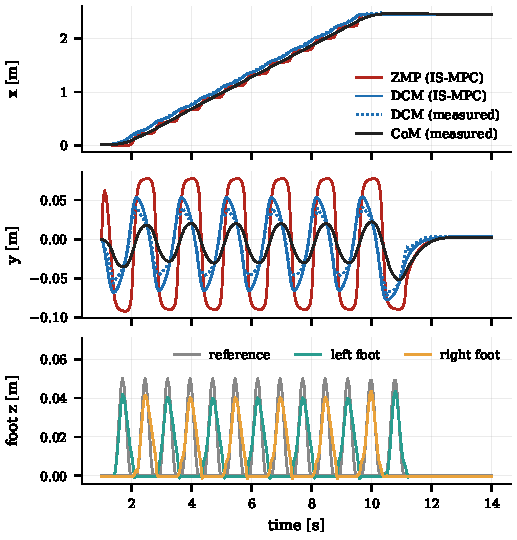
\includegraphics[width=0.74\columnwidth]{figures/walk.pdf}
\caption{Walking at 0.3\,m/s for 8\,s, then stopping. Top and middle: ZMP and DCM planned by the IS-MPC, and DCM and CoM measured on the simulated robot. Bottom: foot height references and measured foot heights.}
\label{fig:walk}
\end{figure}

\subsection{Walking}
Table~\ref{tab:walk} summarizes four commands, each applied for 5\,s (8\,s in the last row) and followed by a two-step stop.
The robot does not fall in any of them, and Fig.~\ref{fig:walk} shows the 0.3\,m/s run.
The measured DCM follows the planned one with an RMS error of 12 to 16\,mm, and the feet track their references within 31\,mm.
The whole-body solve takes 6.7\,ms on average, with 8.2 iterations, and at most 14.2\,ms of the 100\,ms period.
A gait tick takes 2.2\,ms on average, and a touchdown replan (pre-optimization and QP) takes 7.2\,ms on average and at most 11.9\,ms.
The first replan from standing takes 49\,ms, just within the 50\,ms tick.

\begin{table}[t]
\caption{Pushes survived, by DCM shift $d$ (four directions each)}
\label{tab:push}
\centering
\setlength{\tabcolsep}{4pt}
\begin{tabular}{@{}lcccccc@{}}
\toprule
\multicolumn{7}{@{}l}{\emph{Standing}}\\
$d$ [m] & 0.04 & 0.06 & 0.08 & 0.10 & 0.12 & Total\\
\midrule
Push detection on (default) & 4/4 & 4/4 & 4/4 & 1/4$^{\mathrm a}$ & 0/4 & 13/20\\
Push detection off & 4/4 & 4/4 & 2/4 & 1/4 & 0/4 & 11/20\\
\midrule
\multicolumn{7}{@{}l}{\emph{Walking at 0.2\,m/s} (two push instants)}\\
$d$ [m] & \multicolumn{2}{c}{0.05} & \multicolumn{2}{c}{0.08} & & Total\\
\midrule
Default & \multicolumn{2}{c}{7/8} & \multicolumn{2}{c}{6/8} & & 13/16\\
\bottomrule
\multicolumn{7}{@{}l}{$^{\mathrm a}$Two further cases stay up on a tilted foot and are not counted.}
\end{tabular}
\end{table}

\begin{figure}[t]
\centering
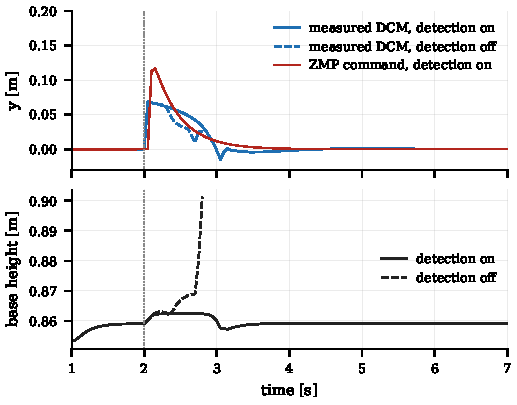
\includegraphics[width=0.7\columnwidth]{figures/push.pdf}
\caption{Lateral push ($d=0.08$\,m, at 2\,s) while standing. With push detection, the gait state is reset to the measured DCM and the standing law moves the ZMP to bring it back. Without it, the robot falls.}
\label{fig:push}
\end{figure}

\subsection{Push recovery}
Table~\ref{tab:push} reports 36 pushes with the default settings: 20 while standing (five magnitudes, four directions) and 16 while walking at 0.2\,m/s (two magnitudes, four directions, two instants of the step cycle).
The robot stays up in 28 cases.
In two of them, lateral pushes of 0.10\,m while standing, it ends balanced on the edge of a foot tilted by 45$^\circ$, which we do not count as a recovery; this leaves 26 of 36.

Closing the loop on the measured DCM helps while standing: with push detection, all pushes of 0.08\,m are recovered, against two of four without it (Fig.~\ref{fig:push}), and a forward push of 0.10\,m is recovered with a capture step.
The failures are directional.
While walking, the three falls are all pushes toward the robot's right; while standing, the failures at 0.10\,m are the backward push and the two lateral ones.

\subsection{What the refiner has to correct}
The results point to three weaknesses, and each one maps to a part of the latent.

\emph{Contact moments.} The CoP ratio in Table~\ref{tab:walk} exceeds 1 in every run, and after strong lateral pushes a stance foot rolls onto its edge.
The OCP treats a stance foot as rigidly fixed, without a limit on the CoP, so both its plan and its feedback ask for ankle moments that the sole cannot transmit.
Adding a wrench-cone penalty to the cost was tried and made walking fail, because the problem relies on these moments to track the lateral CoM reference.
A higher torque weight on the stance ankle reduces the moment the feedback asks for, and a base shift toward the stance foot reduces the moment the plan needs.

\emph{Tracking lag.} The gait generator plans with the LIPM, and the robot lags its reference by 3 to 4\,cm of DCM in single support.
The lag is systematic and depends on the phase of the step, which is what a set-point shift that leads the reference can compensate.

\emph{Reaction to pushes.} The reaction that fails is the one computed for the nominal cost on the unperturbed plan.
Which weights give a reaction that recovers, and in which situation, is what the refiner is meant to learn.
Lateral step limits are narrow ($\pm3.5$\,cm around the nominal foot separation), so part of the lateral failures need a different step and are outside its reach.

\section{Plan}
\label{sec:plan}

Table~\ref{tab:exp} lists the planned experiments.
All of them are evaluated on the protocols of Tables~\ref{tab:walk} and~\ref{tab:push}, repeated with randomized mass, friction and actuation delay.

\begin{table}[t]
\caption{Planned experiments}
\label{tab:exp}
\centering
\setlength{\tabcolsep}{3pt}
\begin{tabular}{@{}cp{0.33\columnwidth}p{0.5\columnwidth}@{}}
\toprule
 & Controller & Question\\
\midrule
B0 & Base controller & Baseline (Section~\ref{sec:results}).\\
B1 & Torque residual with the same torque bound & Does the structure help, compared with an unstructured residual?\\
B2 & Direct scaling of the gains & Does decoding through the solver help, compared with stretching $K$?\\
1 & Refiner, gains only ($a_w$) & Which weights matter, and when?\\
2 & Refiner, set-point only ($a_x$) & Does a base shift reduce the CoP ratio and the tracking lag?\\
3 & Refiner, complete & Are the two parts complementary?\\
\bottomrule
\end{tabular}
\end{table}

The first step is to implement the decoder in Crocoddyl and to calibrate the bounds of the latent, starting from values at which the base behavior is unchanged.
If the refiner fails specifically on delay or contact compliance, this will indicate that the model's dynamics, and not its cost, are the bottleneck.

The MPC runs on the CPU and bounds the training speed.
With the measured times, one simulated second costs about 67\,ms of whole-body solves, 44\,ms of gait ticks and at most 40\,ms of decoding per environment, so $10^8$ refiner steps at 50\,Hz cost on the order of 100 core-hours, which is feasible without a GPU-parallel solver \cite{jeon2025residualmpc}.
After simulation, the controller needs a state estimator and a port to mc\_rtc for experiments on HRP-5P.

\section{Conclusion}
We proposed to refine the feedback policy of a whole-body MPC with a learned policy that acts on the cost weights and on the set-point, using one backward pass of the solver as a decoder.
The refiner stays within gains that are optimal for the model, which makes learning safe and low-dimensional, and it aims at robustness to uncertainty and not at a new motion.
The base controller is implemented and walks in simulation: the reduced model makes the gait generator fast, and its guidance makes the whole-body MPC fast.
The weaknesses that remain, which come from what the two models leave out, map to the two parts of the refiner's latent.

% slightly smaller reference list (small deviation from the IEEE template, to stay within 6 pages)
\begingroup
\renewcommand{\footnotesize}{\fontsize{7.5}{8.6}\selectfont}
\bibliographystyle{IEEEtran}
\bibliography{refs}
\endgroup

\end{document}
